%!TEX root = ../thesis.tex

\section{追従フェーズ}

  追従フェーズの概要を\figref{Fig:RobotGuidance_following_system}に示す.追従フェーズでは,学習フェーズで獲得したモデルを用いる.ここでは,2DLiDARを使用せず,代わりに深層学習器の出力がロボットの行動に影響を与える.つまり,2DLiDARの反射強度に基づくルールベース制御器の出力ではなく,画像を入力とした深層学習器の出力がロボットの行動を決定する.

  \vspace{0.5cm}

  \begin{figure}[h]
    \centering
    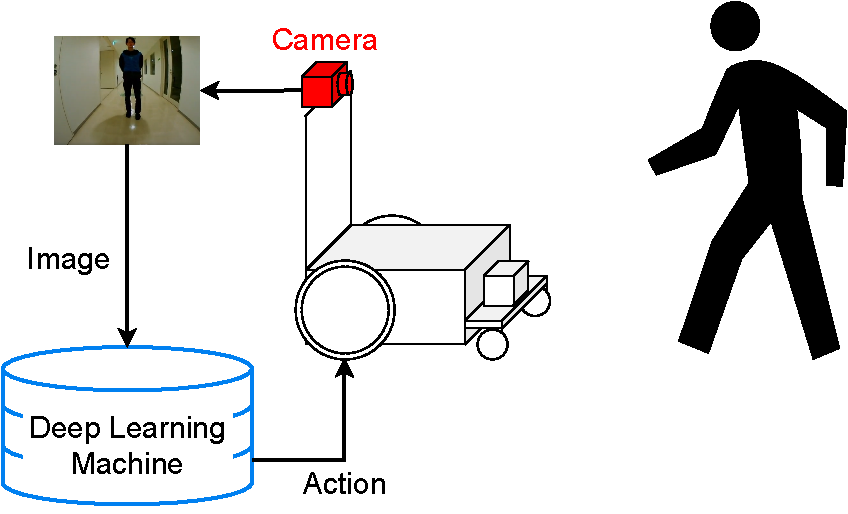
\includegraphics[keepaspectratio, scale=0.45] {images/pdf/RobotGuidance_test_system}
    \captionsetup{justification=raggedright} % キャプションを左寄せに
    \caption{Proposed method in the test phase}
    \label{Fig:RobotGuidance_following_system}
  \end{figure}

  \vspace{0.5cm}

  \begin{figure}[h]
    \centering
    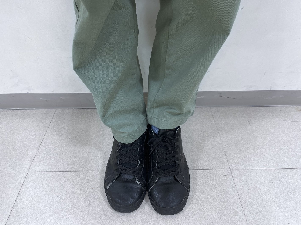
\includegraphics[keepaspectratio, scale=0.55] {images/pdf/RobotGuidance_test_phase_leg}
    \captionsetup{justification=raggedright} % キャプションを左寄せに
    \caption{Without retroreflective tape}
    \label{Fig:RobotGuidance_following_phase_leg}
  \end{figure}

\newpage
